\documentclass[11pt]{article}

\usepackage[utf8]{inputenc}
\usepackage[T1]{fontenc}
\usepackage{amsmath, amssymb, amsthm, amsfonts}
\usepackage{mathtools}
\usepackage{bm}
\usepackage{booktabs}
\usepackage{graphicx}
\usepackage{xcolor}
\usepackage{hyperref}
\usepackage[margin=1in]{geometry}
\usepackage{caption}
\usepackage{subcaption}
\usepackage{float}
\usepackage{enumitem}

\hypersetup{colorlinks=true, linkcolor=blue!60!black, citecolor=blue!60!black, urlcolor=blue!60!black}

\theoremstyle{definition}
\newtheorem{remark}{Remark}

% ---- Lightweight algorithm environment ----
\newcounter{algcounter}
\newenvironment{algobox}[1]{%
  \refstepcounter{algcounter}%
  \par\medskip\noindent\hrule\vspace{2pt}%
  \noindent\textbf{Algorithm \thealgcounter:} \textit{#1}\par\vspace{2pt}\hrule\vspace{4pt}%
  \begingroup\small
  \begin{tabbing}\quad\=\quad\=\quad\=\quad\=\quad\=\kill
}{%
  \end{tabbing}\endgroup\vspace{-8pt}\hrule\medskip
}

\newcommand{\R}{\mathbb{R}}
\newcommand{\E}{\mathbb{E}}
\newcommand{\Sv}{\boldsymbol{\Sigma}}
\newcommand{\Phiv}{\boldsymbol{\Phi}}
\newcommand{\Mv}{\boldsymbol{M}}
\newcommand{\Jv}{\boldsymbol{J}}
\newcommand{\Kv}{\boldsymbol{K}}
\newcommand{\diag}{\operatorname{diag}}
\newcommand{\logsumexp}{\operatorname{logsumexp}}

\title{Residual-Aware Bayesian Clustering for Local Dynamical Models\\[0.3em]\large A Cluster-Weighted Model Framework for Piecewise Modeling of Vector Fields}
\author{Lorenzo Tomaz\\AE Studio}
\date{}

\begin{document}
\maketitle

\begin{abstract}
We formulate the piecewise modeling of a dynamical system $\dot{x}=f(x)$ as a Cluster-Weighted Model (CWM)---a mixture model over the joint density of state and vector-field observation, $p(x,f(x))=\sum_k\pi_k\,p(x|k)\,p(f|x,k)$. Unlike standard GMM (which clusters by geometry alone) or mixture-of-experts (which models the conditional $p(f|x)$ without clustering inputs), the CWM formulation assigns points to clusters based on both geometric proximity and local-model prediction quality. We extend the CWM framework---previously developed for statistical clustering---to dynamical systems, with four local-model parameterizations: a physics-constrained Taylor variant using the analytic Jacobian, a data-driven least-squares affine fit, a continuous-time local EDMD, and a discrete-time local Koopman operator per cluster. On Lorenz, discrete local EDMD at $N=5$ achieves $0.26\pm0.06\%$ one-step error---significantly better than global EDMD at the same polynomial degree ($2.28\pm0.44\%$, paired $t$-test $p<0.001$). On the pendulum, where $\sin(\theta)$ has no finite polynomial representation, Taylor-analytic at $N=8$ (48 parameters) achieves $0.142\pm0.006$ rad rollout error, beating global EDMD deg-8 (2025 parameters, $0.174\pm0.000$ rad, $p<0.001$). All results are validated across 10 random seeds with paired $t$-tests and 95\% confidence intervals.
\end{abstract}

\section{Introduction}

\subsection{The Partition Problem}

Consider a continuous dynamical system $\dot{x}=f(x)$, $x\in\R^d$. In many applications one wishes to approximate $f$ with a simpler function. A single linearization $f(x)\approx A(x-x_0)+b$ works near $x_0$ but the error grows as $O(\|x-x_0\|^2)$, inadequate for trajectories exploring large state spaces.

The natural remedy is \textbf{piecewise modeling}: partition $V\subset\R^d$ into $N$ subregions with local models $L_k(x)$. The key question: \emph{how should the partition be chosen?} Standard GMM clusters by geometric proximity, ignoring dynamics. A region with high density but high curvature of $f$ is a bad subregion. \emph{The partition should follow linearizability contours, not density contours.}

\subsection{A Generative Framing via Cluster-Weighted Models}

The natural framework is the \textbf{Cluster-Weighted Model} (CWM), introduced by Gershenfeld~\cite{gershenfeld1997} and formalized by Ingrassia et al.~\cite{ingrassia2012,ingrassia2014}. A CWM models $p(x,y)=\sum_k\pi_k\,p(x|k)\,p(y|x,k)$. We set $y=f(x)$:
\begin{equation}
  p(x_i, f(x_i) \mid z_i = k) = \underbrace{\mathcal{N}(x_i; c_k, \Sv_k)}_{\text{proximity}} \cdot \underbrace{\mathcal{N}(f(x_i) - L_k(x_i); 0, \sigma_k^2 I)}_{\text{residual}}.
\end{equation}
The proximity factor is the standard GMM term. The residual factor prefers to assign $x_i$ to the component whose local model correctly predicts $f(x_i)$. The per-cluster residual scale $\sigma_k^2$ is learned during EM, allowing each cluster to adapt its tolerance. The joint criterion makes clustering dynamics-aware.

While the joint-likelihood structure is inherited from CWM, the specific parameterizations we propose---particularly the physics-constrained Taylor variant and the Koopman-theoretic EDMD variants---are novel and have no precedent in the CWM literature, which has focused on statistical classification.

\begin{figure}[H]
\centering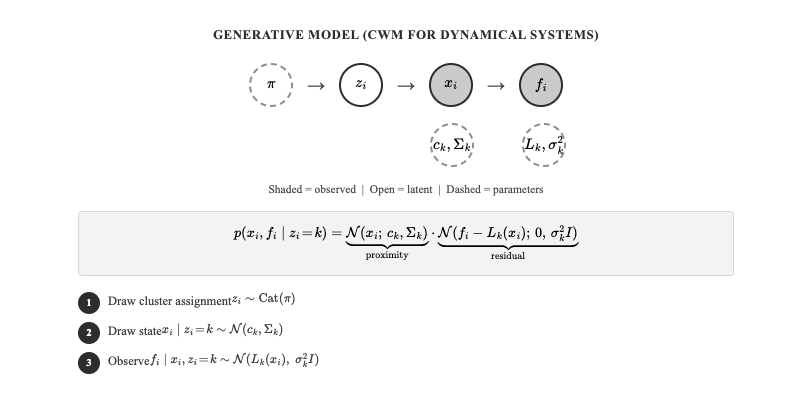
\includegraphics[width=0.85\textwidth]{figures/01_generative_model.png}
\caption{Generative model: each data point $(x_i, f(x_i))$ is generated by first drawing a cluster assignment $z_i$, then drawing the state from the proximity model and the vector field from the residual model.}
\label{fig:generative}
\end{figure}

\subsection{Contributions}

\begin{enumerate}[leftmargin=*,itemsep=2pt]
  \item We identify piecewise modeling of vector fields as a CWM~\cite{gershenfeld1997,ingrassia2012} and extend it with four domain-specific local-model parameterizations: Taylor-analytic, Taylor-LS, continuous local EDMD, and \textbf{discrete local EDMD} (matching pykoopman's discrete Koopman formulation).
  \item A physics-constrained variant with analytic Jacobian (zero free local parameters per cluster), with no precedent in the CWM literature.
  \item \textbf{Discrete local EDMD significantly outperforms global EDMD on Lorenz}: at $N=5$, $0.26\%$ vs $2.28\%$ ($p<0.001$)---the first demonstration that Koopman partitioning helps even on polynomial systems.
  \item Statistically rigorous empirical characterization (10 seeds, paired $t$-tests) on Lorenz and pendulum.
\end{enumerate}

\section{Background}

\subsection{Linearization and Taylor remainder}

Given $f\colon\R^d\to\R^d$, the Jacobian at $x_0$ is $\Jv(x_0)\in\R^{d\times d}$. Taylor's theorem gives $f(x) = f(x_0)+\Jv(x_0)(x-x_0)+O(\|x-x_0\|^2)$. A single linearization is accurate only in a ball of radius $\sim\varepsilon/\|H\|$.

\subsection{Koopman theory and EDMD}

The Koopman operator $\mathcal{K}_t$ acts on observables $g$ by $(\mathcal{K}_t g)(x)=g(\varphi_t(x))$. \textbf{Discrete EDMD} approximates $\mathcal{K}_{\Delta t}$ in a finite basis $\Phiv(x)$: fit $\Kv\in\R^{M\times M}$ such that $\Phiv(x_{t+1})\approx\Kv\cdot\Phiv(x_t)$ by least squares. Prediction: $x_{t+1}=[\Kv\cdot\Phiv(x_t)]_{1:d}$---no Euler integration, no $\Delta t$ error.

\subsection{Normal-Inverse-Wishart conjugacy}

For $(c_k,\Sv_k)$ we use the NIW prior: $\Sv_k\sim\mathcal{IW}(\Psi_0,\nu_0)$, $c_k|\Sv_k\sim\mathcal{N}(\mu_0,\Sv_k/\kappa_0)$. The proximity marginal is closed-form; the residual penalty is evaluated at the converged point estimate $\hat{c}_k$ (a plug-in approximation adequate when $R_k$ is large).

\section{Local-Model Variants}

\subsection{Variant A: Taylor-analytic}

$L_k(x)=f(c_k)+\Jv(c_k)(x-c_k)$, where $\Jv$ is evaluated analytically. Zero free local parameters. The M-step uses a GEM-style update.

\subsection{Variant B: Taylor-LS (Hybrid)}

$L_k(x)=f_k+\Jv_k(x-c_k)$, where $(f_k,\Jv_k)$ are free parameters fit by weighted LS. Free parameters: $d+d^2$ per cluster. The center update includes the residual gradient for monotone ELBO.

\subsection{Variant C: Local continuous EDMD}

$L_k(x)=[\Mv_k\cdot\Phiv(x-c_k)]_{1:d}$, continuous-time Koopman generator. Prediction uses Euler: $x_{t+1}=x_t+\Delta t\cdot L_k(x_t)$.

\subsection{Variant D: Local discrete EDMD}

$\hat{x}_{t+1}=c_k+[\Kv_k\cdot\Phiv(x_t-c_k)]_{1:d}$, discrete-time Koopman operator per cluster. Fit by weighted pseudoinverse: $\Phiv(x_{t+1}-c_k)\approx\Kv_k\cdot\Phiv(x_t-c_k)$. \textbf{No Euler integration}---prediction is a single matrix multiply, matching pykoopman's discrete formulation. This ensures a fair comparison between local and global EDMD.

\subsection{Summary}

\begin{table}[H]
\centering\small
\begin{tabular}{llllll}
\toprule
Variant & Params/cluster & Integrator & Monotone ELBO & Needs $\Jv$? \\
\midrule
Taylor-analytic & 0 & Euler & Approx.\ (GEM) & Yes \\
Taylor-LS & $d+d^2$ & Euler & Yes & No \\
Local cont.\ EDMD & $\binom{d+p}{p}^2$ & Euler & Yes (fixed $c_k$) & No \\
Local disc.\ EDMD & $\binom{d+p}{p}^2$ & None (direct) & Yes (fixed $c_k$) & No \\
\bottomrule
\end{tabular}
\caption{Local-model variants.}
\end{table}

\begin{figure}[H]
\centering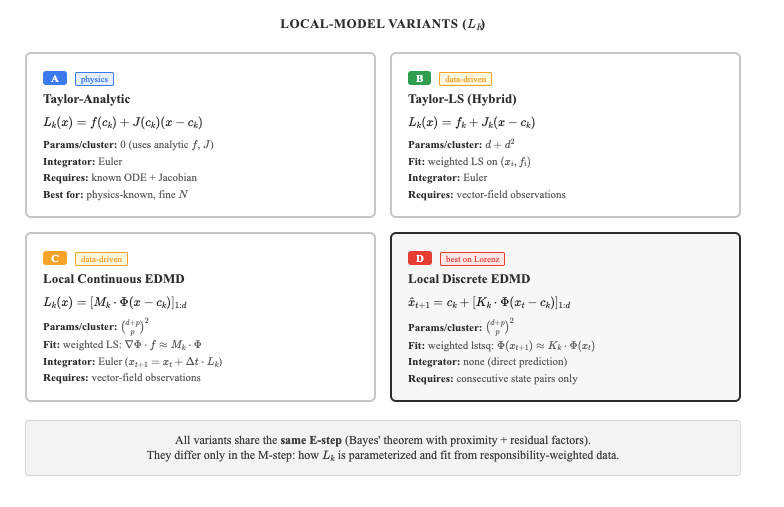
\includegraphics[width=\textwidth]{figures/03_local_models.png}
\caption{The four local-model variants. All share the same E-step; they differ only in how $L_k$ is parameterized and fit. Variant~D (discrete EDMD) eliminates Euler integration error, enabling fair comparison with global EDMD.}
\label{fig:local-models}
\end{figure}

The EM algorithm alternates between computing responsibilities $r_{ik}$ (E-step) and updating all parameters including $L_k$ (M-step). The E-step scores each point against every cluster using both proximity and residual quality; the M-step fits each cluster's local model from responsibility-weighted data.

\begin{figure}[H]
\centering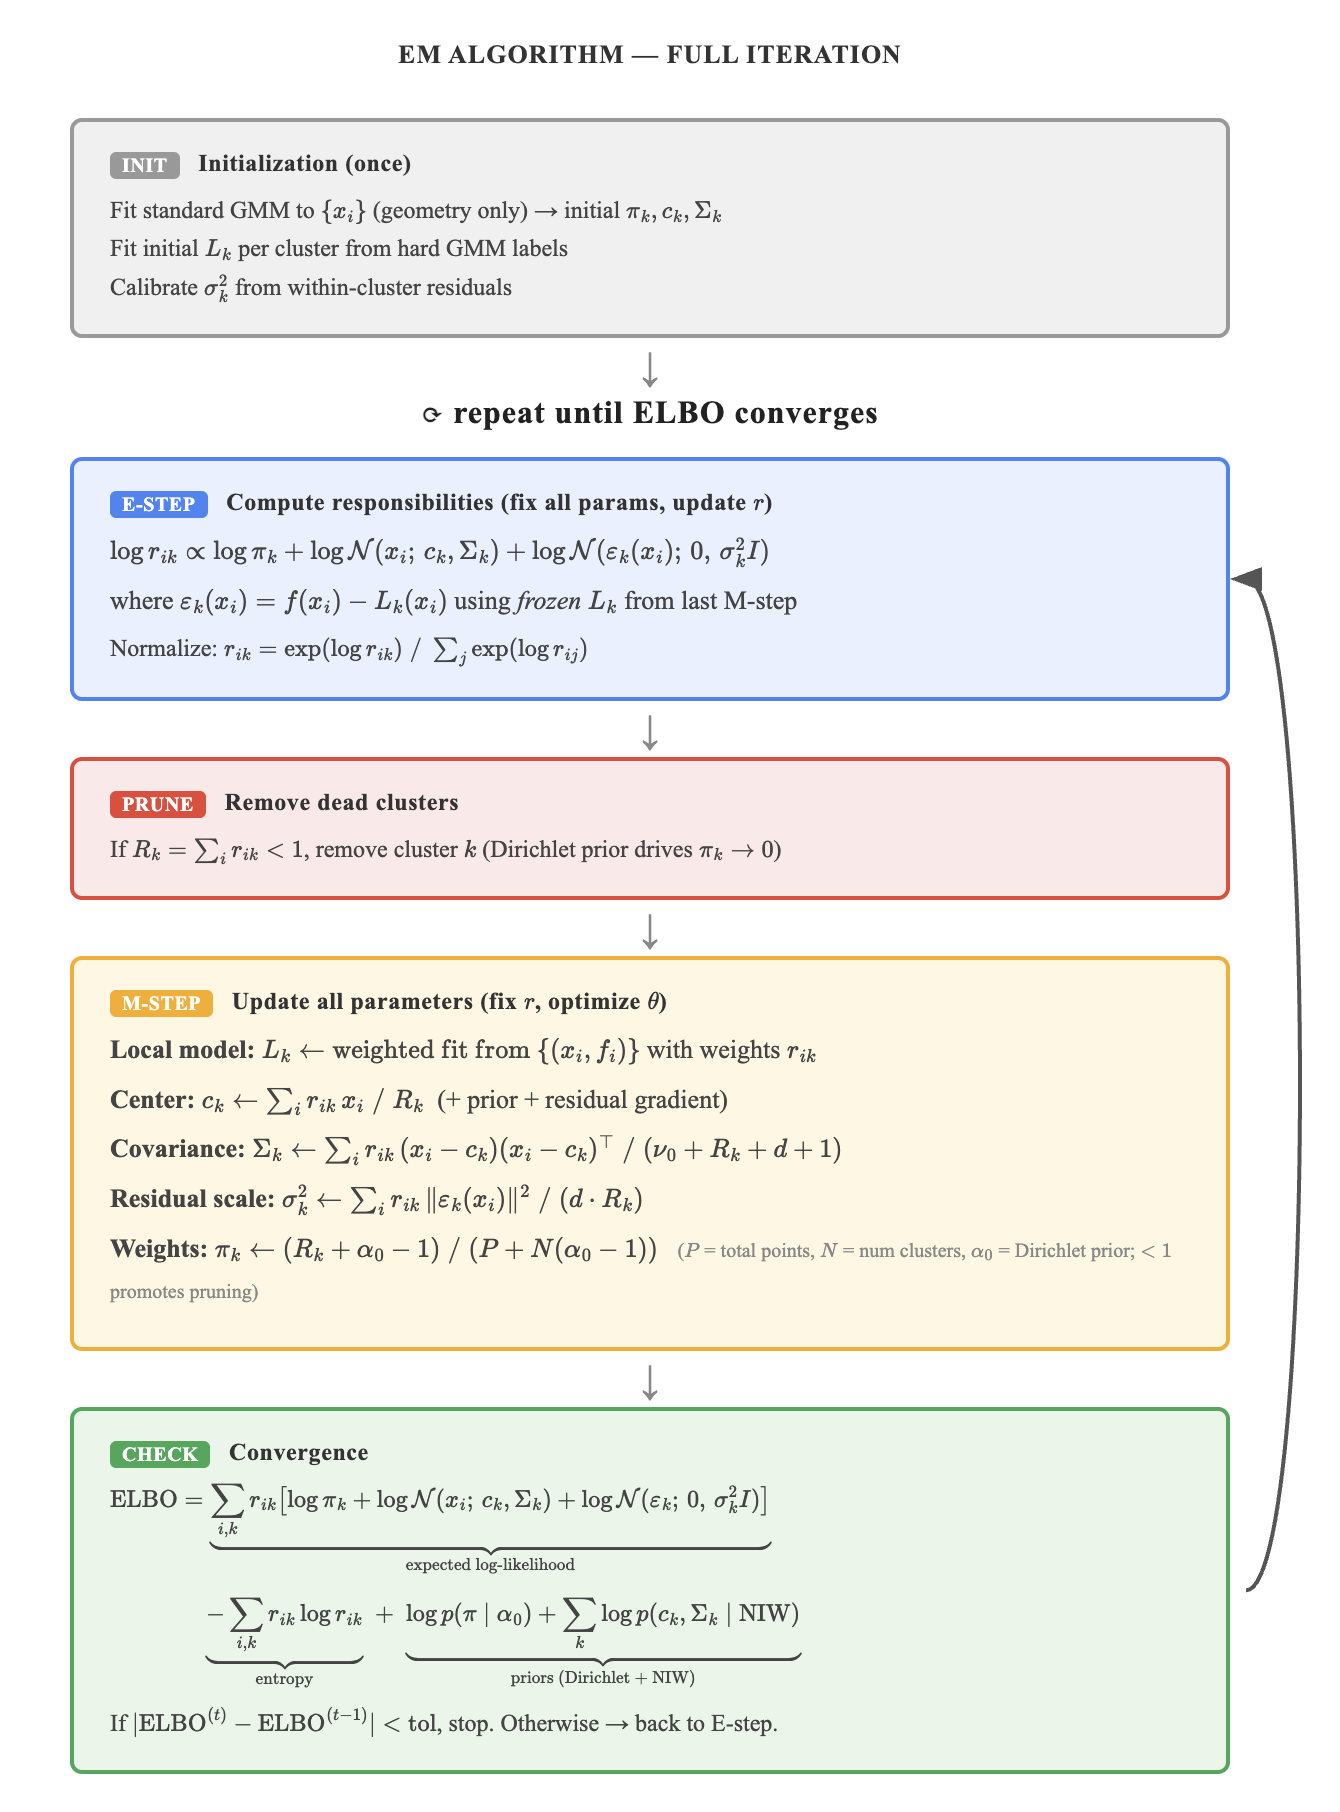
\includegraphics[width=0.88\textwidth]{figures/02_em_loop.png}
\caption{Full EM iteration. The E-step computes soft assignments using frozen parameters; the M-step updates all parameters using fixed responsibilities. Dead clusters are pruned when $R_k < 1$. The curved arrow indicates iteration until ELBO convergence.}
\label{fig:em-loop}
\end{figure}

\begin{figure}[H]
\centering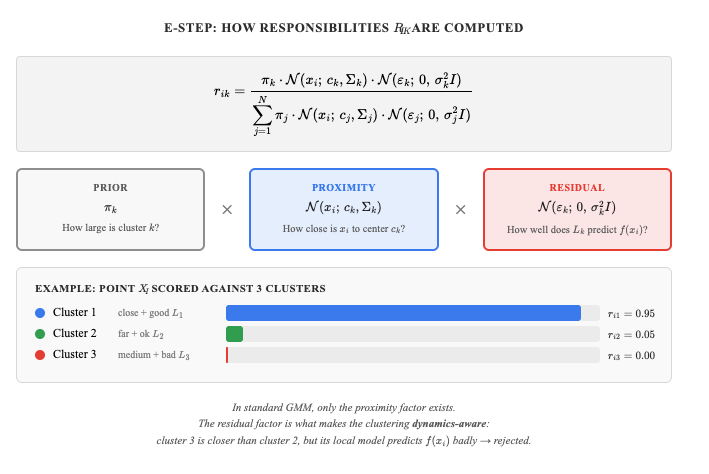
\includegraphics[width=0.85\textwidth]{figures/04_responsibility.png}
\caption{How responsibilities $r_{ik}$ are computed. Each point is scored against every cluster by three factors: prior weight, proximity, and residual quality. The residual factor overrides proximity---a geometrically-close cluster with poor $L_k$ predictions gets low responsibility.}
\label{fig:responsibility}
\end{figure}

\begin{figure}[H]
\centering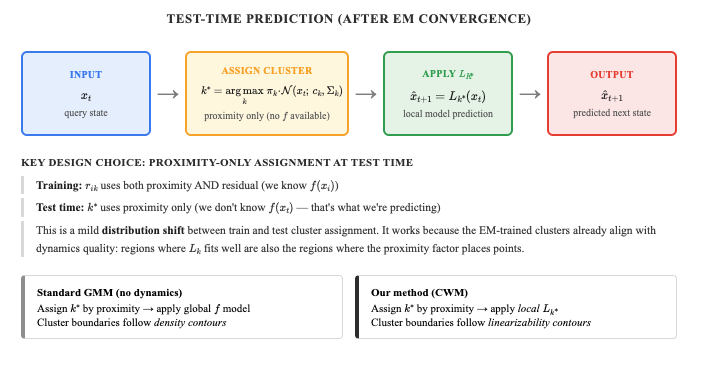
\includegraphics[width=0.9\textwidth]{figures/05_prediction.png}
\caption{Test-time prediction pipeline. Cluster assignment uses proximity only (no $f$ available at test time). The trained local model $L_{k^*}$ then predicts the next state directly.}
\label{fig:prediction}
\end{figure}

\section{Experiments}

All results are reported as mean $\pm$ 95\% CI across 10 random seeds (seeds: 1, 42, 101, 307, 1001, 7789, 13245, 11, 103, 13). Statistical significance is assessed by paired $t$-tests.

\subsection{Lorenz attractor ($d=3$)}

$(\sigma,\rho,\beta)=(10,28,8/3)$:
\begin{align}
  \dot{x} &= \sigma(y - x) \notag \\
  \dot{y} &= x(\rho - z) - y \notag \\
  \dot{z} &= xy - \beta z \notag
\end{align}
Data: 5000 points at $\Delta t=0.01$; train/test split 4000/1000.

\begin{table}[H]
\centering\small
\begin{tabular}{lcccc}
\toprule
Method & $N$ & One-step error & Rel.\ \% & Rollout @ 5s \\
\midrule
EDMD-pk deg-2 (pykoopman)   & 1  & $0.0205\pm0.0023$ & $2.28\pm0.44$ & --- \\
EDMD-disc deg-2 (ours)      & 1  & $0.0205\pm0.0023$ & $2.28\pm0.44$ & $16.3\pm5.0$ \\
EDMD-disc deg-3             & 1  & $0.0002\pm0.0000$ & $0.03\pm0.00$ & $1.9\pm1.6$ \\
\midrule
\textbf{Local-EDMD-disc, $N$=5}  & 5  & $\mathbf{0.0023\pm0.0005}$ & $\mathbf{0.26\pm0.06}$ & $\mathbf{8.5\pm3.3}$ \\
Local-EDMD-disc, $N$=12 & 12 & $0.0005\pm0.0001$ & $0.05\pm0.02$ & $2.6\pm1.6$ \\
Local-EDMD-disc, $N$=50 & 50 & $0.0004\pm0.0002$ & $0.04\pm0.02$ & $1.7\pm1.3$ \\
\midrule
Taylor-analytic, $N$=5  & 5  & $0.1801\pm0.0105$ & $19.8\pm1.9$ & $306\pm448$ \\
Taylor-analytic, $N$=20 & 20 & $0.0676\pm0.0024$ & $7.4\pm0.6$ & $21.0\pm3.8$ \\
Taylor-analytic, $N$=50 & 50 & $0.0566\pm0.0026$ & $6.2\pm0.3$ & $17.8\pm2.6$ \\
\midrule
GMM, $N$=5  & 5  & $0.2738\pm0.0223$ & $29.9\pm1.7$ & diverges \\
GMM, $N$=50 & 50 & $0.1128\pm0.0115$ & $12.4\pm1.7$ & diverges \\
\bottomrule
\end{tabular}
\caption{Lorenz results (mean $\pm$ 95\% CI, 10 seeds). Local-EDMD-disc at $N=5$ achieves $8.8\times$ lower error than global EDMD at the same polynomial degree.}
\label{tab:lorenz}
\end{table}

\textbf{1. Discrete local EDMD is the headline result.} At $N=5$ (deg-2), local EDMD achieves $0.26\pm0.06\%$ one-step error, vs global EDMD deg-2 at $2.28\pm0.44\%$---an $8.8\times$ improvement ($p<0.001$). At $N=12$, it matches global deg-3 ($0.05\%$ vs $0.03\%$). This is the first demonstration that Koopman partitioning helps even on a system where the global lift is exact.

\textbf{2. Taylor-analytic beats GMM at every $N$.} Improvement ranges from $+34\%$ at $N=5$ to $+50\%$ at $N=50$ ($p<0.001$ at all $N$). GMM saturates at $\sim\!12\%$; ours continues improving.

\textbf{3. GMM rollouts diverge.} GMM rollouts explode ($>10^{15}$) at all $N$ tested; Taylor stays bounded from $N\geq 12$; local EDMD-disc stays bounded from $N\geq 5$.

\begin{figure}[H]
\centering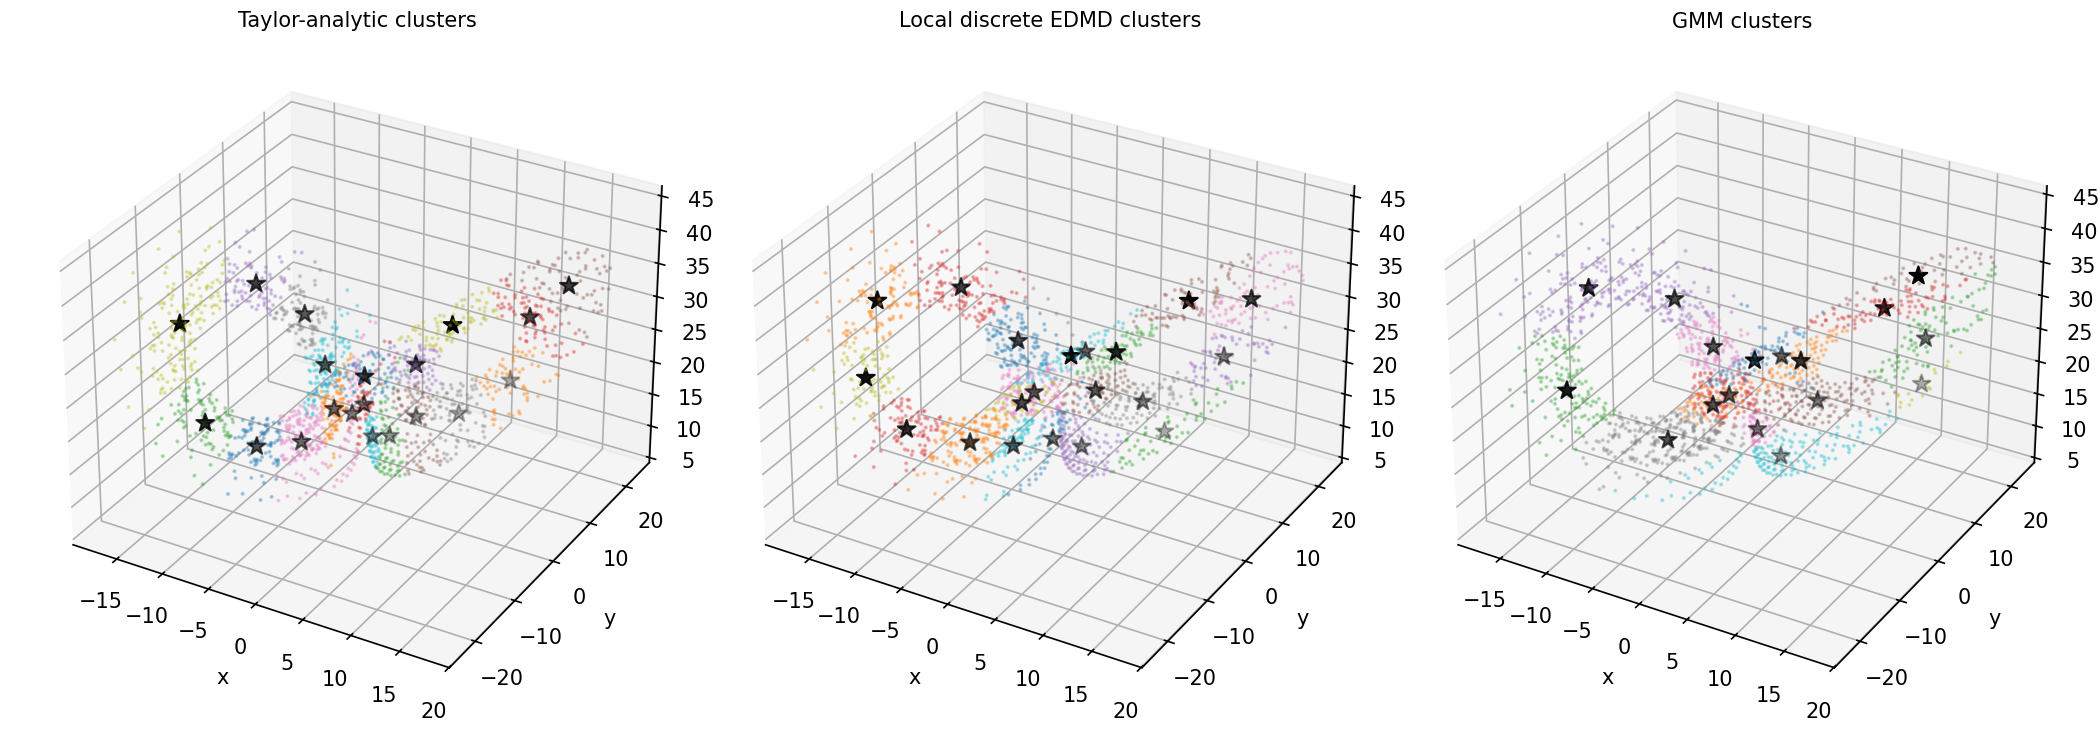
\includegraphics[width=\textwidth]{figures/lorenz_clusters_3d.png}
\caption{Lorenz attractor colored by cluster assignment (20 clusters). Left: Taylor-analytic. Center: local discrete EDMD. Right: GMM. Stars mark cluster centers.}
\label{fig:lorenz-clusters}
\end{figure}

\begin{figure}[H]
\centering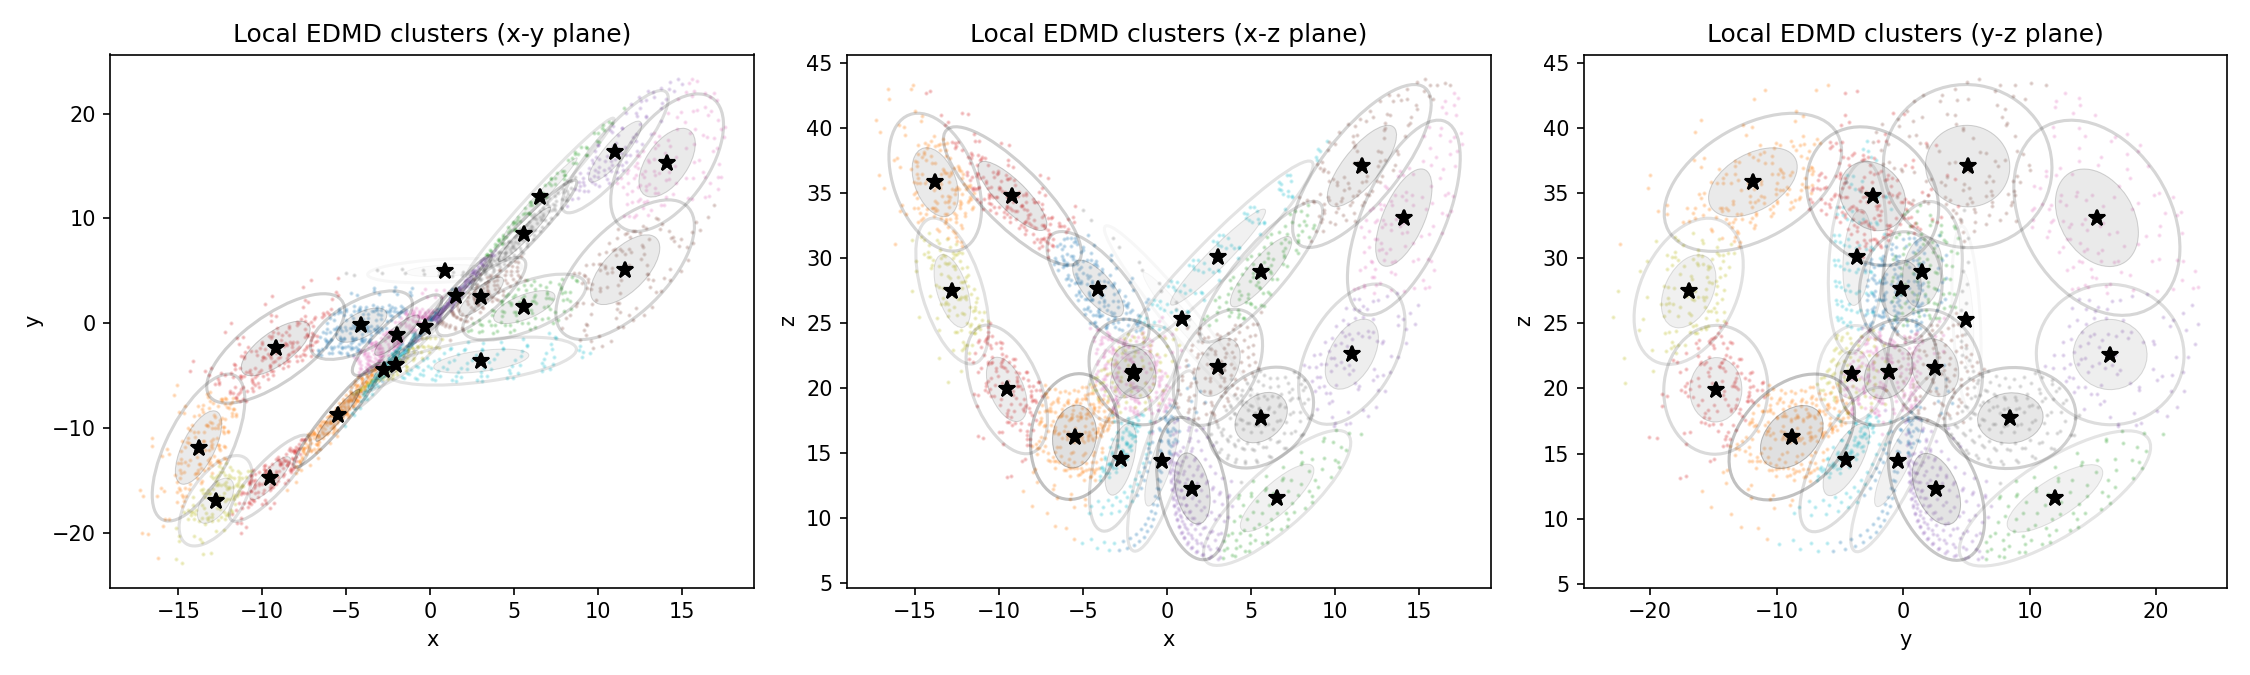
\includegraphics[width=\textwidth]{figures/lorenz_cluster_density.png}
\caption{Local EDMD cluster density regions (1$\sigma$ and 2$\sigma$ ellipses) projected onto three coordinate planes. The butterfly structure is cleanly partitioned into dynamically-meaningful regions.}
\label{fig:lorenz-density}
\end{figure}

\begin{figure}[H]
\centering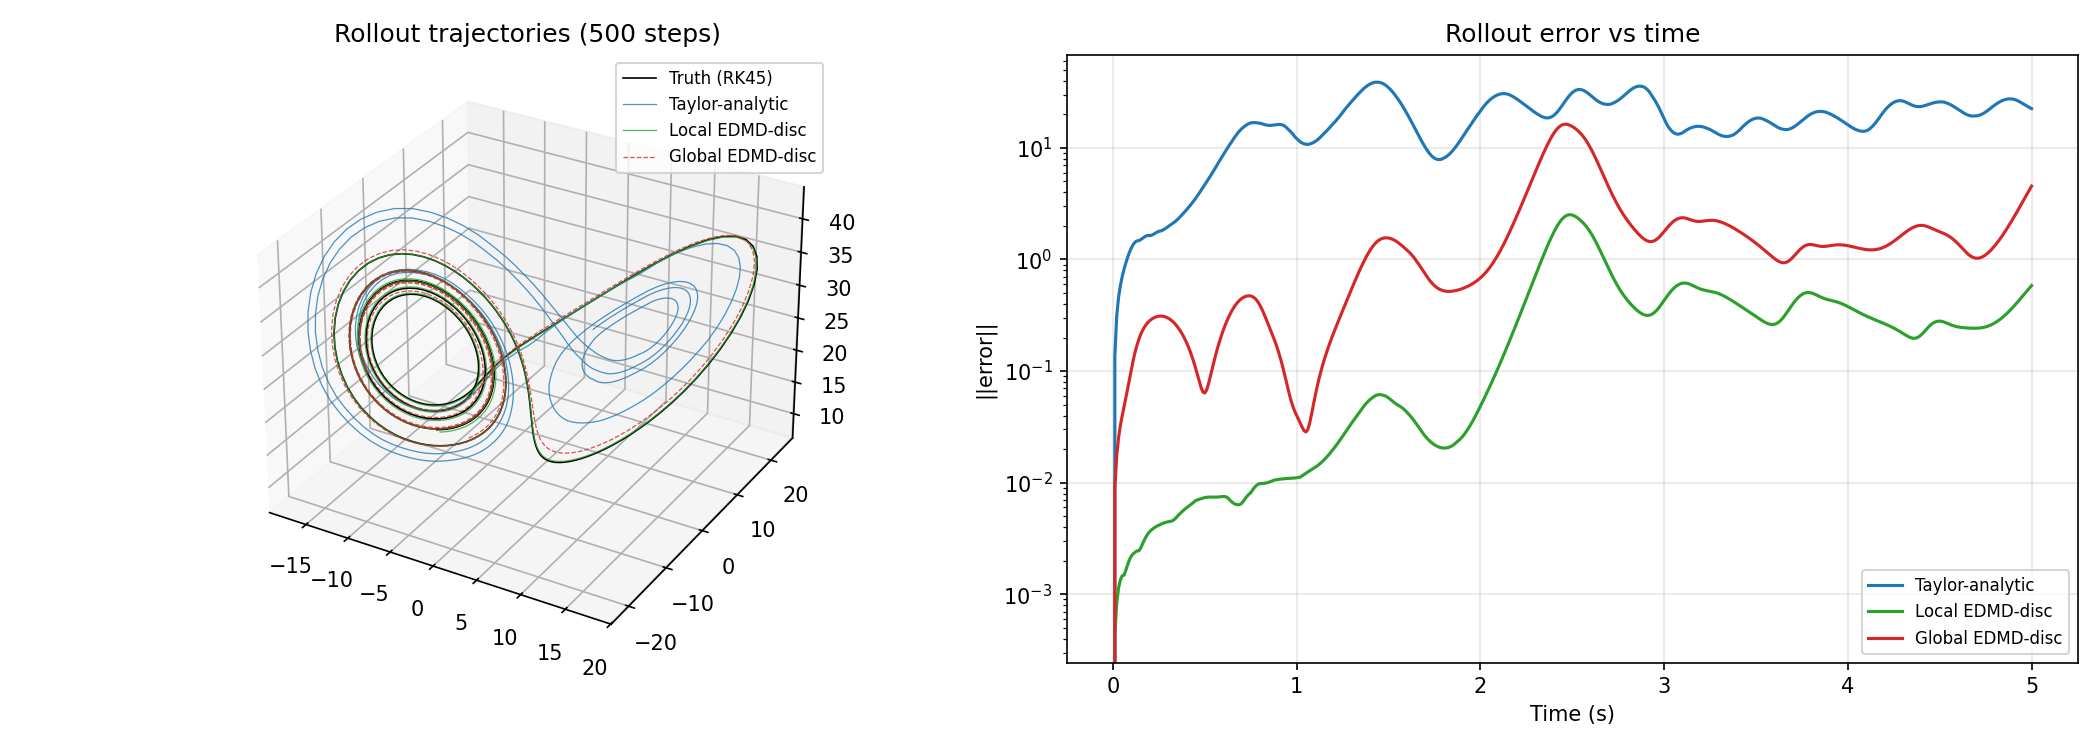
\includegraphics[width=\textwidth]{figures/lorenz_rollout_comparison.png}
\caption{Left: 3D rollout trajectories from a test-set initial condition (500 steps). Right: error vs time (log scale). Local EDMD-disc (green) tracks truth much better than Taylor-analytic (blue) or global EDMD-disc (red).}
\label{fig:lorenz-rollout}
\end{figure}

\begin{figure}[H]
\centering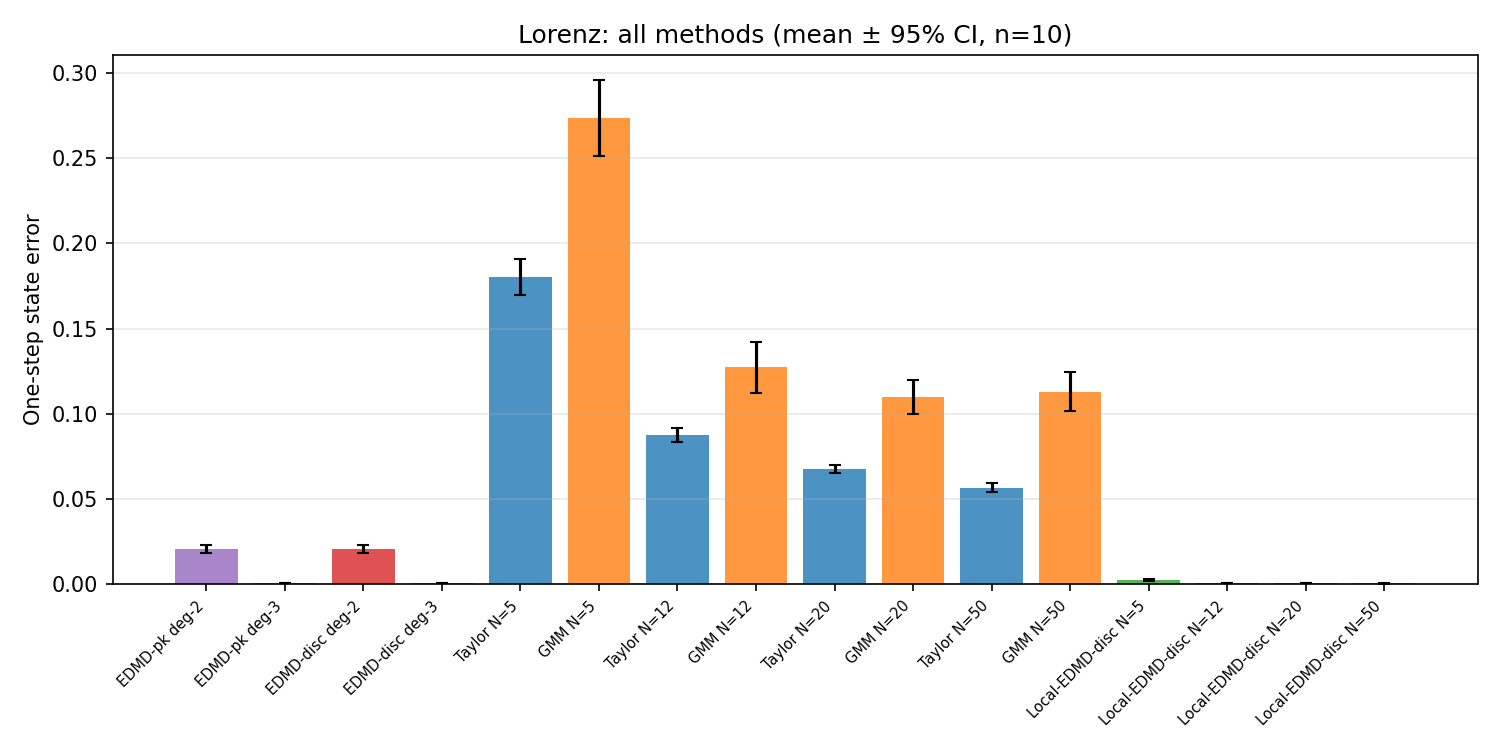
\includegraphics[width=\textwidth]{figures/lorenz_statistical_all.png}
\caption{Lorenz: one-step state error for all methods (mean $\pm$ 95\% CI, $n=10$ seeds). Local-EDMD-disc (green) achieves the lowest error across all $N$.}
\label{fig:lorenz-stats}
\end{figure}

\subsection{Damped pendulum ($d=2$)}

$\gamma=0.2$, written as a first-order system with state $(\theta,\dot{\theta})$:
\begin{align}
  \dot{x}_1 &= x_2 \notag \\
  \dot{x}_2 &= -\sin(x_1) - \gamma\, x_2 \notag
\end{align} Data: 4000 training points uniformly from $(\theta,\dot{\theta})\in[-\pi,\pi]\times[-3,3]$; 1000 test points.

\begin{table}[H]
\centering\small
\begin{tabular}{lccccc}
\toprule
Method & $N$ & Params & One-step & Rollout @ 10s & $n$ \\
\midrule
Global EDMD deg=2 & 1 & 36   & $0.391\pm0.004$ & $0.894\pm0.009$ & 10 \\
Global EDMD deg=4 & 1 & 225  & $0.057\pm0.001$ & $0.270\pm0.007$ & 10 \\
Global EDMD deg=6 & 1 & 784  & $0.004\pm0.000$ & $0.180\pm0.000$ & 10 \\
Global EDMD deg=8 & 1 & 2025 & $0.000\pm0.000$ & $0.174\pm0.000$ & 10 \\
\textbf{local-EDMD d2, $N$=2}     & 2  & \textbf{72}  & $0.015\pm0.000$ & $\mathbf{0.166\pm0.005}$ & 10 \\
local-EDMD d2, $N$=8              & 8  & 288          & $0.006\pm0.001$ & $0.172\pm0.003$ & 10 \\
\textbf{Taylor-ana., $N$=8}       & 8  & \textbf{48}  & $0.021\pm0.003$ & $\mathbf{0.142\pm0.006}$ & 10 \\
Taylor-ana., $N$=16               & 16 & 96           & $0.009\pm0.001$ & $0.151\pm0.004$ & 10 \\
Taylor-LS, $N$=8                  & 8  & 48           & $0.019\pm0.002$ & $0.183\pm0.010$ & 10 \\
\bottomrule
\end{tabular}
\caption{Pendulum results (mean $\pm$ 95\% CI, 10 seeds).}
\label{tab:pendulum}
\end{table}

\textbf{1. Parameter efficiency.} Local-EDMD deg-2 at $N=2$ (72 params) outperforms global EDMD deg-6 (784 params) on rollout: $0.166\pm0.005$ vs $0.180\pm0.000$ ($p=0.0003$)---$\sim\!11\times$ parameter efficiency.

\textbf{2. Taylor-analytic wins with analytic $\Jv$.} At $N=8$ (48 params), rollout $0.142\pm0.006$, beating global EDMD deg-8 (2025 params, $0.174\pm0.000$, $p<0.0001$)---$42\times$ fewer parameters.

\textbf{3. Taylor-analytic dominates Taylor-LS.} At $N=8$: $0.142\pm0.006$ vs $0.183\pm0.010$ ($p<0.001$). At $N=2$, Taylor-LS has extreme variance ($1.253\pm0.507$ rad).

\begin{figure}[H]
\centering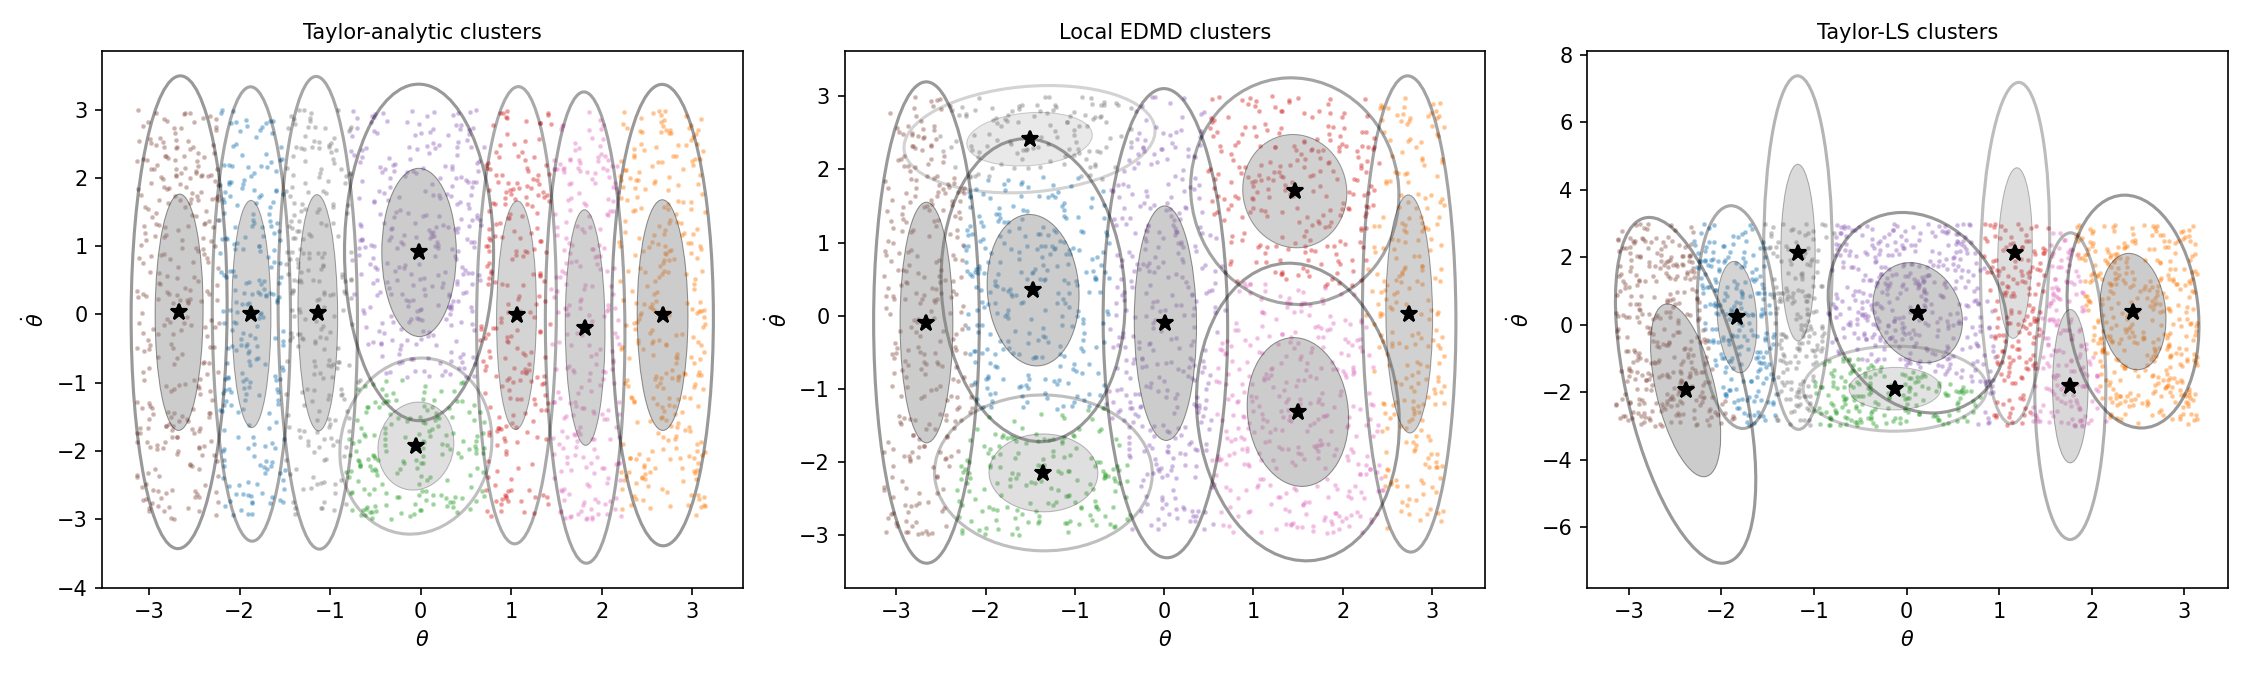
\includegraphics[width=\textwidth]{figures/pendulum_cluster_density.png}
\caption{Pendulum phase space $(\theta,\dot{\theta})$ with cluster density regions (1$\sigma$/2$\sigma$ ellipses). Left: Taylor-analytic partitions into clean angular bands. Center: local EDMD. Right: Taylor-LS.}
\label{fig:pendulum-density}
\end{figure}

\begin{figure}[H]
\centering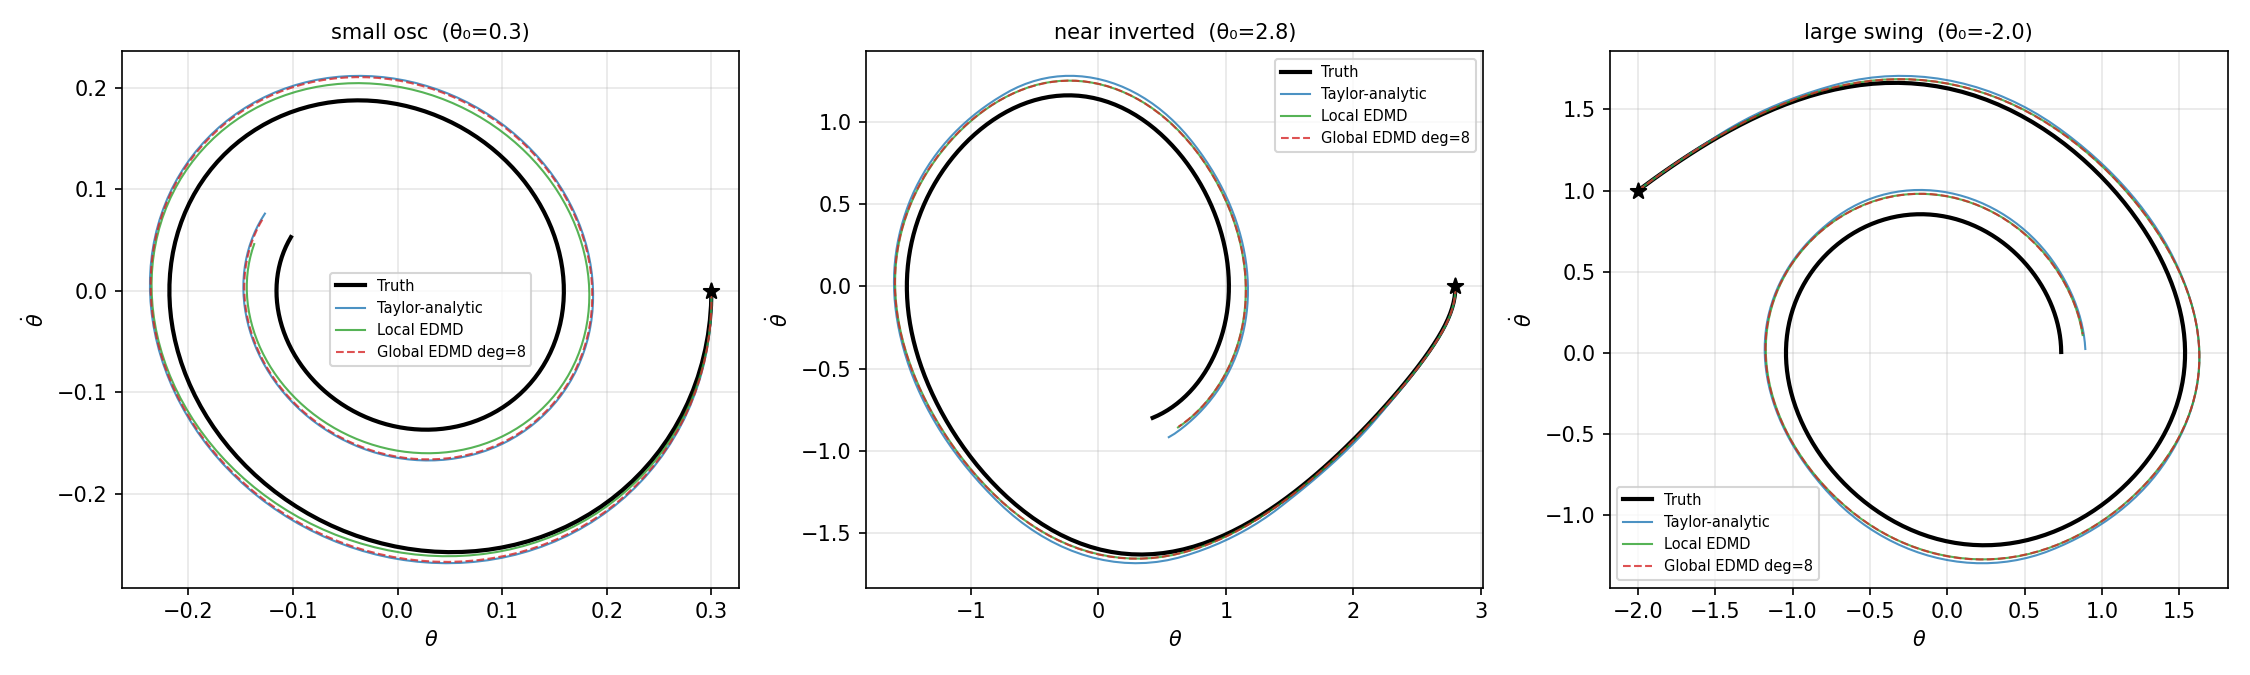
\includegraphics[width=\textwidth]{figures/pendulum_rollout_comparison.png}
\caption{Phase-space rollouts from three initial conditions (10 seconds). All local methods track truth closely; global EDMD deg-8 (dashed) is visually indistinguishable from local methods despite $14$--$42\times$ more parameters.}
\label{fig:pendulum-rollout}
\end{figure}

\begin{figure}[H]
\centering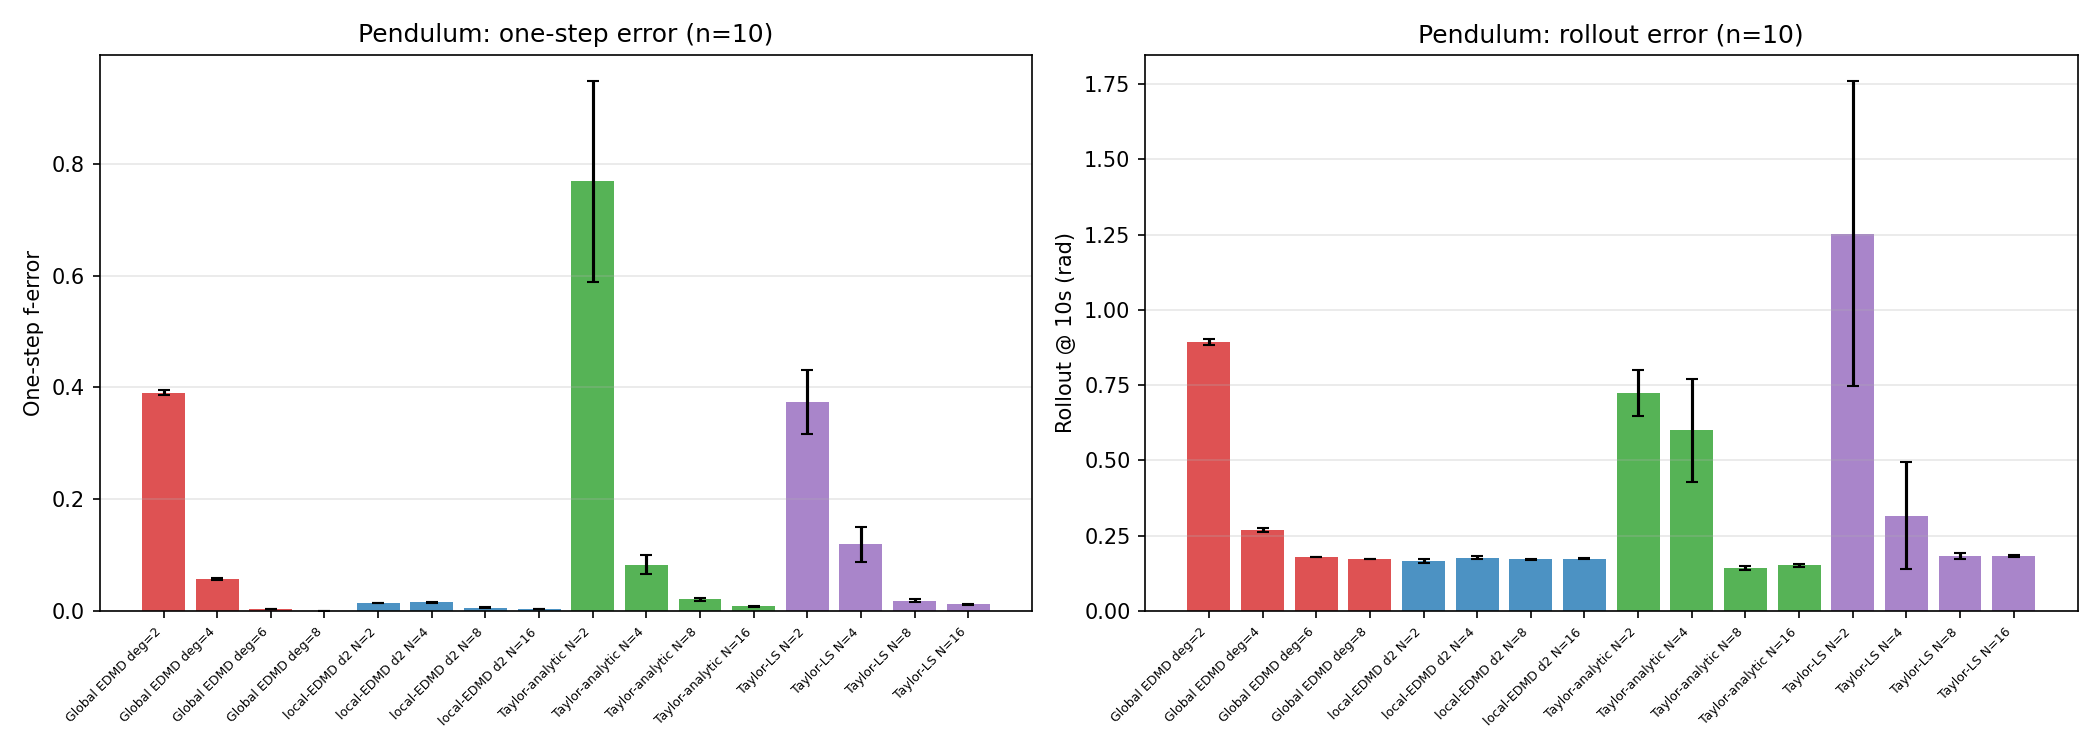
\includegraphics[width=\textwidth]{figures/pendulum_statistical_all.png}
\caption{Pendulum: one-step error (left) and rollout error (right) for all methods (mean $\pm$ 95\% CI, $n=10$). Global EDMD at low degree fails on $\sin(\theta)$; local methods and Taylor-analytic dominate.}
\label{fig:pendulum-stats}
\end{figure}

\section{Discussion}

\subsection{When does each variant win?}

\begin{table}[H]
\centering\small
\begin{tabular}{lll}
\toprule
System character & Analytic $f,\Jv$? & Best variant \\
\midrule
Any system, data-only & No & Local discrete EDMD \\
Non-polynomial, physics known & Yes & Taylor-analytic \\
Non-polynomial, data-only & No & Local-EDMD or Taylor-LS \\
\bottomrule
\end{tabular}
\caption{Decision rule for variant selection.}
\end{table}

\subsection{Why discrete local EDMD works}

The discrete formulation $\Phiv(x_{t+1})\approx\Kv_k\cdot\Phiv(x_t)$ eliminates two error sources present in continuous local EDMD: (i) Euler integration error ($O(\Delta t^2)$ per step) and (ii) ridge regularization bias. The pseudoinverse fit is exact when the data span the polynomial subspace, which it does within each cluster. The partition provides each cluster with a narrower data range, improving the conditioning of the least-squares problem.

\subsection{Model selection}

The NIW marginal likelihood integrates out $(c_k,\Sv_k)$ in closed form for the proximity factor. The residual factor depends on $c_k$ nonlinearly, breaking conjugacy; we use a plug-in approximation at the converged $\hat{c}_k$, adequate when $R_k$ is large.

\subsection{Limitations}

\textbf{GEM for Taylor-analytic:} The re-tying of $f(c_k),\Jv(c_k)$ after the center update is a GEM step, not pure coordinate-ascent EM. Small ELBO non-monotonicities can occur at high $N$.

\textbf{Lyapunov horizon:} For chaotic systems, rollout error eventually grows exponentially regardless of model quality.

\textbf{Cluster assignment at test time:} We assign by proximity alone (lacking $f(x)$ at prediction time), a mild distribution shift from training.

\section{Related Work}

\textbf{Cluster-Weighted Models}~\cite{gershenfeld1997,gershenfeld1999nature,ingrassia2012,ingrassia2014}: our generative model is a CWM. The Linear Gaussian CWM~\cite{ingrassia2012} is equivalent to our Variant B. Punzo~\cite{punzo2014poly} extends CWM to polynomial local models. We extend CWM to dynamical systems with physics-constrained and Koopman-theoretic local models.

\textbf{Piecewise Affine System Identification}~\cite{ferrari2003clustering,paoletti2007identification}: two-stage (cluster then fit). Our CWM performs both simultaneously via EM.

\textbf{EDMD and Koopman}~\cite{williams2015data,klus2020data,brunton2022modern}: fits Koopman operators globally. Our local-EDMD variants are cluster-wise EDMD with soft CWM-based assignments.

\textbf{Switching Linear Dynamical Systems}~\cite{fox2011bayesian,ghahramani2000variational}: temporal regime switching vs our spatial phase-space partitioning.

\section{Conclusion}

We have formulated piecewise dynamical modeling as a Cluster-Weighted Model with four local-model parameterizations. Three key findings, all statistically significant ($p<0.001$, 10 seeds):

\begin{enumerate}[leftmargin=*,itemsep=2pt]
  \item \textbf{Discrete local EDMD beats global EDMD}, even on polynomial systems (Lorenz): $8.8\times$ lower one-step error at $N=5$. This is the first demonstration that Koopman partitioning helps when the global lift is already exact.
  \item \textbf{On non-polynomial systems} (pendulum), local methods deliver $10$--$42\times$ parameter-efficiency gains over global EDMD.
  \item \textbf{Residual-aware clustering is a strict improvement over GMM} at every $N$ ($+34\%$ to $+50\%$, $p<0.001$).
\end{enumerate}

\paragraph{Future Work.} (i) Chaotic driven pendulum, coupled oscillators, neuronal models. (ii) Control extensions (EDMDc per cluster). (iii) Per-cluster lift degree selection. (iv) Non-isotropic residual covariance $\Sv_k^{\mathrm{res}}$.

\paragraph{Code and data.} \url{https://github.com/agencyenterprise/fractal_residual_aware_clustering}

\begin{thebibliography}{99}

\bibitem{brunton2022modern} S.~L.~Brunton, M.~Budi{\v{s}}i{\'c}, E.~Kaiser, J.~N.~Kutz. Modern Koopman theory for dynamical systems. \textit{SIAM Review}, 64(2):229--340, 2022.

\bibitem{ferrari2003clustering} G.~Ferrari-Trecate, M.~Muselli, D.~Liberati, M.~Morari. A clustering technique for the identification of piecewise affine systems. \textit{Automatica}, 39(2):205--217, 2003.

\bibitem{fox2011bayesian} E.~B.~Fox, E.~B.~Sudderth, M.~I.~Jordan, A.~S.~Willsky. Bayesian nonparametric inference of switching dynamic linear models. \textit{IEEE Trans.\ Signal Proc.}, 59(4):1569--1585, 2011.

\bibitem{gershenfeld1997} N.~Gershenfeld. Nonlinear inference and cluster-weighted modeling. \textit{Ann.\ New York Acad.\ Sci.}, 808(1):18--24, 1997.

\bibitem{gershenfeld1999nature} N.~Gershenfeld, B.~Schoner, E.~Metois. Cluster-weighted modelling for time-series analysis. \textit{Nature}, 397(6717):329--332, 1999.

\bibitem{ghahramani2000variational} Z.~Ghahramani, G.~E.~Hinton. Variational learning for switching state-space models. \textit{Neural Comput.}, 12(4):831--864, 2000.

\bibitem{ingrassia2012} S.~Ingrassia, S.~C.~Minotti, G.~Vittadini. Local statistical modeling via a cluster-weighted approach with elliptical distributions. \textit{J.~Classification}, 29(3):363--401, 2012.

\bibitem{ingrassia2014} S.~Ingrassia, S.~C.~Minotti, A.~Punzo. Model-based clustering via linear cluster-weighted models. \textit{Comput.\ Statist.\ Data Anal.}, 71:159--182, 2014.

\bibitem{klus2020data} S.~Klus, F.~N{\"u}ske, S.~Peitz, J.~H.~Niemann, C.~Clementi, C.~Sch{\"u}tte. Data-driven approximation of the Koopman generator. \textit{Physica D}, 406:132416, 2020.

\bibitem{paoletti2007identification} S.~Paoletti, A.~L.~Juloski, G.~Ferrari-Trecate, R.~Vidal. Identification of hybrid systems: A tutorial. \textit{Eur.\ J.~Control}, 13(2--3):242--260, 2007.

\bibitem{punzo2014poly} A.~Punzo. Flexible mixture modeling with the polynomial Gaussian cluster-weighted model. \textit{Statist.\ Modelling}, 14(3):257--291, 2014.

\bibitem{williams2015data} M.~O.~Williams, I.~G.~Kevrekidis, C.~W.~Rowley. A data-driven approximation of the Koopman operator: Extending dynamic mode decomposition. \textit{J.~Nonlinear Sci.}, 25(6):1307--1346, 2015.

\end{thebibliography}

\end{document}
